\chapter{Zoznam použitých skratiek}

\begin{center}
AVAD - Acoustic Voice Actividy Detection\\
CLI - Command-Line Interface\\
CNN - Convolutional neural network\\
DCNN - Deep convolutional neural network\\
DNN - Deep neural network\\
EBGM  - Elastic Bunch Graph Matching\\
GMM - Gausian Mixture Model\\
GUI - Graphical User Interface\\
HCI  - Human–Computer Interaction\\
HoG - Histogram of oriented gradients\\
SVM - Support-vector machine\\
VAD - Voice Activity Detection\\
VVAD - Visual Voice Actividy Detection

\end{center}

\chapter{Teoretický prehľad}

\section{Human-Computer Interaction}
HCI - Human-Computer Interaction (interakcia človek počítač), je medziodborová disciplína, ktorá skúma problematiku interakcie a komunikácie medzi človekom a počítačom.
Vznikla na prelome 70. a 80. rokov dvadsiateho storočia, v dobe, keď začali vznikať prvé osobné počítače.
HCI v sebe spája veľa oborovPOZNodborov?, ktoré na prvý pohľad nemajú nič spoločné. 
Ak sa však chceme zaoberať vytváraním používateľských rozhraní, kľúčové sú nasledujúce disciplíny: informatika, ergonómia, umenie, design, psychológia, kognitívna psychológia, lingvistika, sociológia, filozofia, antropológia, fyziológia, umelá inteligencia, inžinierstvo, kognitívna veda, etika, estetika a. i.

Informatika sa v oblasti HCI zameriava najmä na design a tvorbu informačných systémov a ich rozhraní tak, aby boli co najjednoduchšie a najintuitívnejšie pre špecifickú skupinu používateľov.
HCI skúma aj vnímanie, správanie a informačné potreby koncového používateľa. 
Hlavným cieľom HCI je dosiahnuť lepšiu použiteľnosť a intuitívnosť informačných systémov aj pre menej odborných používateľov. \cite{HCI}

\section{Vývoj HCI}
V tejto časti popíšeme historický vývoj komunikácie medzi človekom a počítačom.

\subsection{CLI}
Od polovice 60. rokov sa CLI - Command-Line Interface (príkazový riadok) používa ako hlavný spôsob komunikácie človeka s počítačom.
Používateľ zadáva príkazy pomocou klávesnice, výsledky vidí na monitore väčšinou v textovej podobe.
Používanie CLI pokračuje v 70. a 80. rokoch systémoch OpenVMS, Unix a osobných počítačoch MS-DOS, CP/M a Apple DOS.
Pre skúseného používateľa má CLI veľa výhod, uvedieme niektoré z nich:
\begin{itemize}
	\item rýchlosť a efektívnosť,
	\item možnosť použitie skriptov,
	\item história príkazov,
	\item nie je potrebná myš, stačí klávesnica,...
\end{itemize}
Ale pre menej skúseného používateľa prináša veľa nevýhod, napríklad:
\begin{itemize}
	\item prostredie je veľmi neintuitívne a striktné,
	\item nemožnosť použitia myši, ...
\end{itemize}
Aj v dnešnej dobe je CLI často používané, najmä medzi používateľmi linuxu, na spravovanie serverov a podobne.

\subsection{GUI}
S príchodom väčšieho grafického výkonu vzniká GUI - Graphical User Interface (Grafické používateľské rozhranie). 
Okrem klávesnice sa používa počítačová myš a vznikajú okná.
Oproti CLI má GUI veľké výhody pre neskúseného používateľa:
\begin{itemize}
	\item intuitívnosť,
	\item rýchlosť - v špecifických prípadoch (napr. presúvanie súborov), ...
\end{itemize}
Často ale môže nastať prípad, keď sú niektoré nastavenia príliš hlboko v systéme a pomocou GUI sa k nim nie je možné dostať.
V dnešnej dobe je GUI najpoužívanejším typom HCI na osobných počítačoch.

\subsection{NUI}
S príchodom nových technológií (smatrfónov, virtuálnej reality, ...) sa do popredia začína dostávať NUI - Natural User Interface (Prirodzené používateľské rozhranie).
Pomocou NUI dokáže používateľ úplne prirodzene, priamo a intuitívne interagovať s počítačom.
Príkladom NUI, s ktorým sa už asi každý stretol, je používanie gest na dotykových obrazovkách.
Ďalšie príklady NUI je možné vidiet na nasledujúcich obrázkoch \ref{pic-GoogleHome}, \ref{pic-Microrobotics} a \ref{pic-calcFlow}.

\begin{figure}[H]
	\begin{center}
		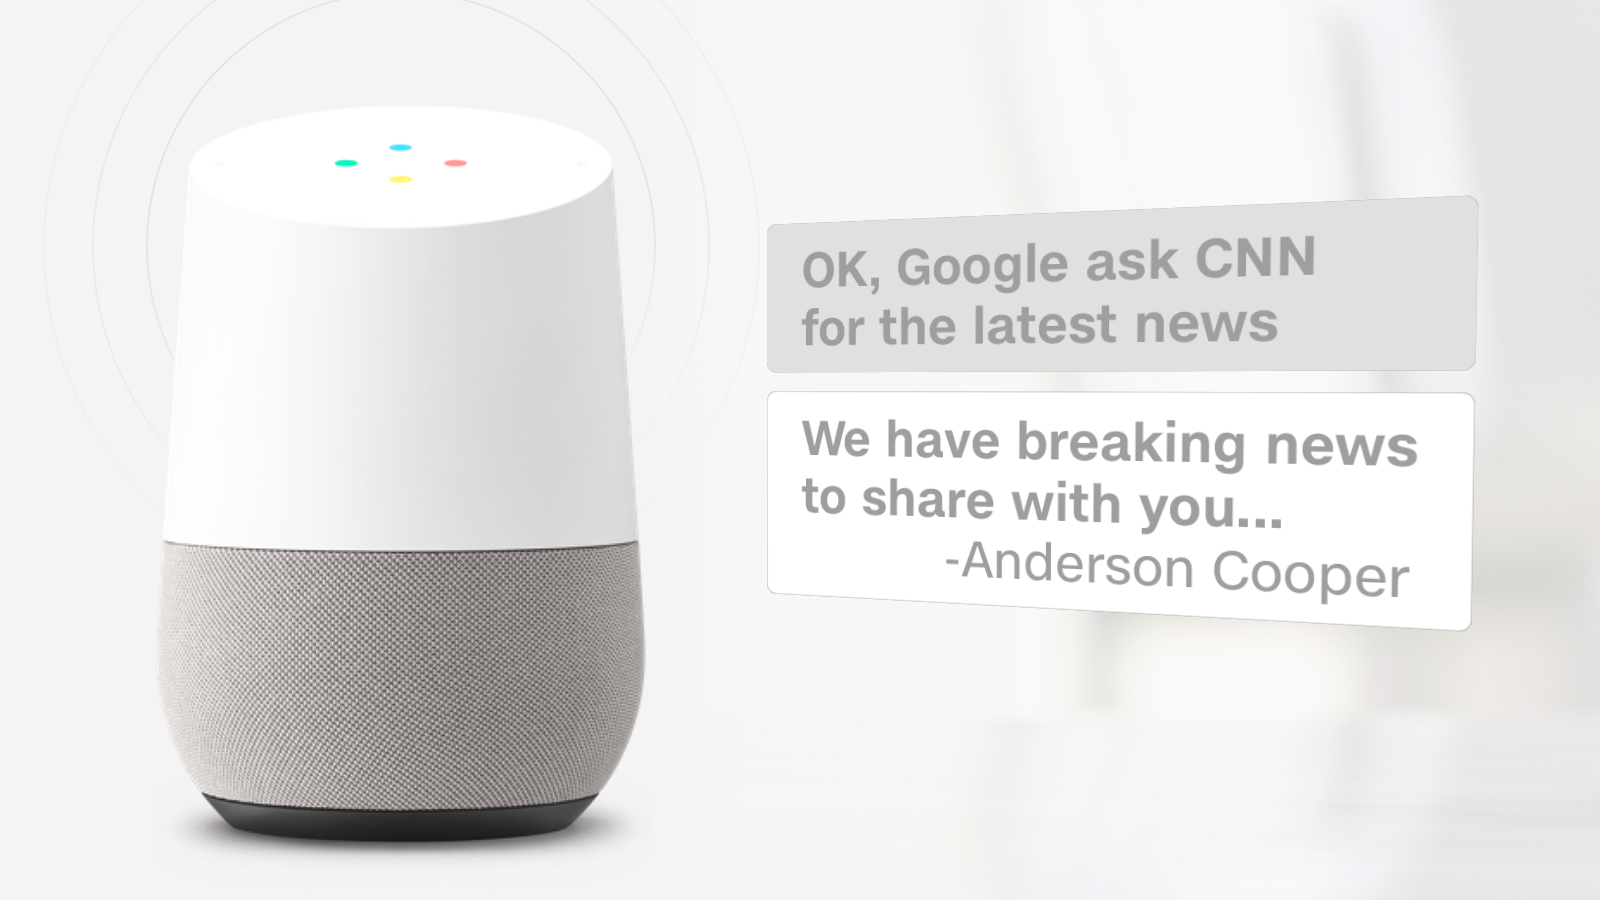
\includegraphics[height=5cm]{pics/googleHome.jpg}
		\caption{Google Home - Inteligentný domáci asistent, s ktorým sa komunikuje pomocou hlasových príkazov.
		 \cite{GoogleHome}}
		\label{pic-GoogleHome}
	\end{center}
\end{figure}

\begin{figure}[H]
	\begin{center}
		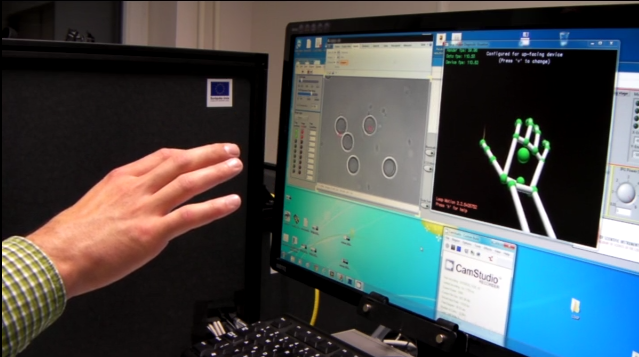
\includegraphics[height=5cm]{pics/Microrobotics.png}
			\caption{Manipulácia objektov pomocou optickej pinzety, kontrolovaná pozíciou prstov.
			\cite{Microrobotics}}
		\label{pic-Microrobotics}
	\end{center}
\end{figure}

\begin{figure}[H]
	\begin{center}
		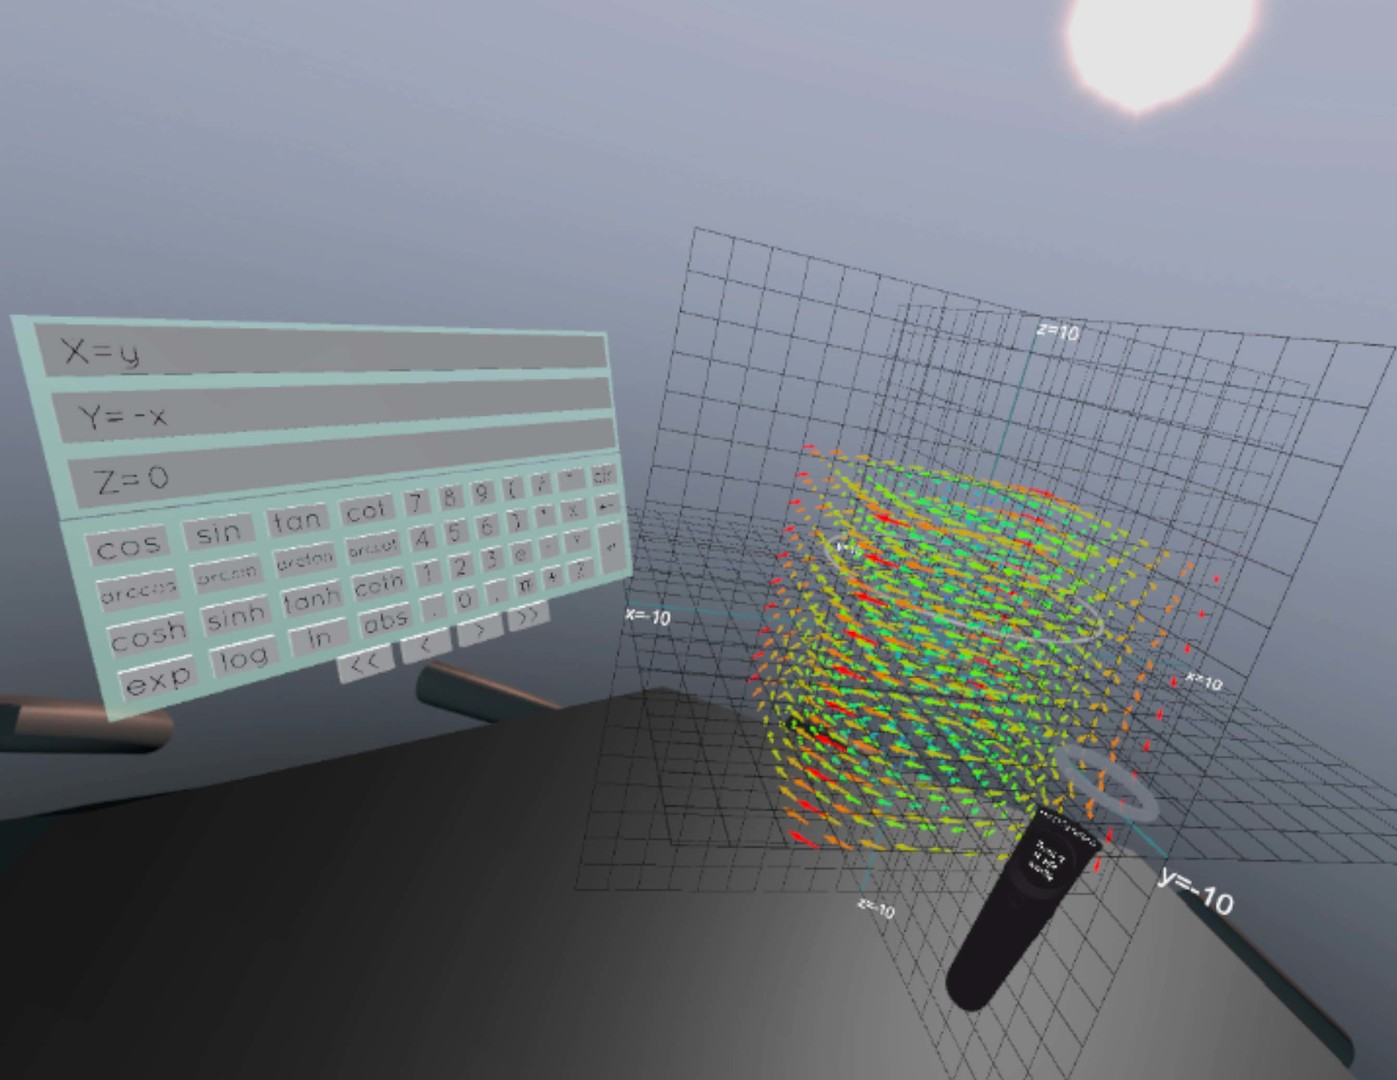
\includegraphics[height=5cm]{pics/calcFlow.jpg}
		\caption{Používanie aplikácie Calcflow vo virtuálnej realite. 
		 \cite{calcFlow}}
		\label{pic-calcFlow}
	\end{center}
\end{figure}

\chapter{Motivácia a ciele}
Jedným z hlavných motívov, prečo vznikla táto práca bola nasledujúca situácia. 

Predstavme si situáciu konferenčného hovoru. 
Jeden z účastníkov potrebuje niečo urobiť, no jeho aktivita by bola hlučná, čím by rušil ostatných účastníkov a teda si vypne mikrofón. 
Samozrejme, neskôr keď chce niečo povedať, nezapne mikrofón a ostatní ho nepočujú.

Ako by sme sa mohli popísanej situácií vyhnúť? 
Čo tak zapínať a vypínať mikrofón automaticky podla toho, či človek sediaci pred kamerou rozpráva alebo nerozpráva.
Jedným z riešení by mohla byť detekcia reči (Voice activity detection - VAD) pomocou mikrofónu (Acoustic Voice Actividy Detection - AVAD).
Toto riešenie však nemusí byť najpresnejšie, napríklad by nemuselo detegovať tichý hlas alebo by detegovalo nechcený šum a podobne.
Vhodným zlepšením by mohlo byť zlúčenie AVAD s VAD pomocou obrazu webovej kamery (Visual Voice Actividy Detection - VVAD).
Naštudovali sme niekoľko existujúcich riešení, ktoré sú popísané v nasledujúcej kapitole.

Ďalším krokom pri vypracovávaní tejto práce, bude implementovanie vlastného riešenia VAD inšpirovaného existujúcimi riešeniami a snaha o jeho implementáciu do existujúceho videokonferenčného systému. 

\chapter{Riešenia VAD}
V nasledujúcich odsekoch ukážeme niekoľko existujúcich riešení.
Zameriame sa na použité technológie, dosiahnuté výsledky a problémy, ktoré majú uvedené riešenia.\\

V \cite{aoki2007voice} riešia VAD u šoféra v aute.
Reč detegujú zo zvuku pomocou Gausian mixture model (GMM).
Túto detekciu kombinujú s VVAD.
Kvôli odfiltrovaniu nepriaznivých odleskov a nedostatku svetla v noci používajú infračervenú kameru.
Z šedo-tónového obrazu získavajú obrysy pier, pomocou Elastic Bunch Graph Matching (EBGM).
Ukážku získaného obrysu pier je možné vidieť na \ref{pic-EBGM}. 

\begin{figure}[H]
	\begin{center}
		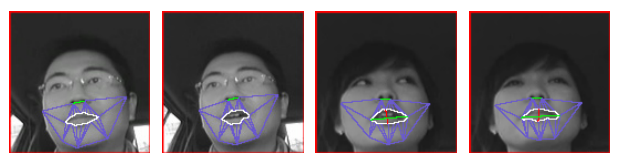
\includegraphics[height=4cm]{pics/EBGM.png}
		\caption{Získavaný obrys pier pomocou EBGM.
		 \cite{aoki2007voice}}
		\label{pic-EBGM}
	\end{center}
\end{figure}

Z pier určujú pomer ich výšky a šírky.
Získaný pomer má výhodu v nezávislosti od vzdialenosti tváre od kamery.
Obrázok \ref{pic-pery} vysvetľuje prečo sa pomer mení, len keď človek rozpráva.

\begin{figure}[H]
	\begin{center}
		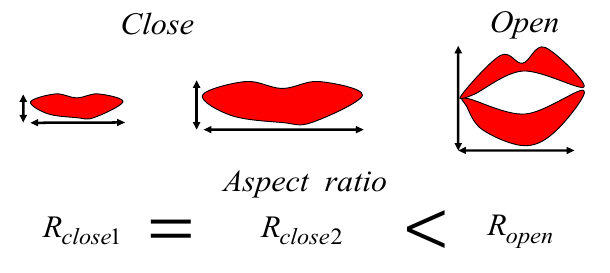
\includegraphics[height=3.5cm]{pics/pery.png}
		\caption{Pomer výšky a šírky pier sa zmení len keď sa ústa otvárajú a zatvárajú.
		 \cite{aoki2007voice}}
		\label{pic-pery}
	\end{center}
\end{figure}

Navrhnutú metódu testovali tak, že šofér (raz muž a raz žena) prečítal 100 názvov japonských miest.
Testovaná metóda priemerne zlepšuje detekciu reči o 40\% oproti použitiu len AVAD.  
Získane výsledky možno vidieť v tabuľke \ref{tab-results}.

\begin{table}[H]
	\begin{center}
		\begin{tabular}{|c|c|c|c|r|}
			\hline
			& Všetky zdetegovania reči & Správne zdetegovania reči & Úspešnosť & Presnosť \\
			\hline
			muž & 106 & 100 & 100\% & 94,33\%\\
			\hline
			žena & 118 & 100 & 100\% & 84,75\%\\
			\hline
		\end{tabular}
	\end{center}
	\caption{Výsledky testovania metódy v práci \cite{aoki2007voice}}
	\label{tab-results}
\end{table}

Nevýhodou metódy je to, že funguje len pri pohľade spredu. V článku sa nepíše nič o rýchlosti ich riešenia.\\

V \cite{vieriu2014real} sa zaoberajú detegovaním reči z jednoduchej webovej kamery. 
Najprv orežú snímky videa na oblasť pier.
Snímky prevedú do šedotónovej oblasti, vyrežú 200 náhodných oblastí a urobia rozdiel všetkých snímok a prvého. 
Takto vedia modelovať zmeny vo vzhľade podľa rozdielov v čase.
Z každého rozdielu počítajú štatistické koeficienty priemer, smerodajnú odchýlku a priemer nad prvou deriváciou. 
Aplikovaním popísaného postupu vytvorili tréningovú množinu o veľkosti 130000.
Následne natrénovali klasifikátor Random Forest s veľkosťou 20 stromov a maximálnou hĺbkou 10. 
Random Forest porovnávali s klasifikátorom Random Ferns. 
Random Ferns dosahovali pri rôznych nastaveniach parametrom stále horšie výsledky ako Random Forests.
Porovnanie týchto dvoch metód je na obrázku \ref{pic-ferns&forests}.

\begin{figure}[H]
	\begin{center}
		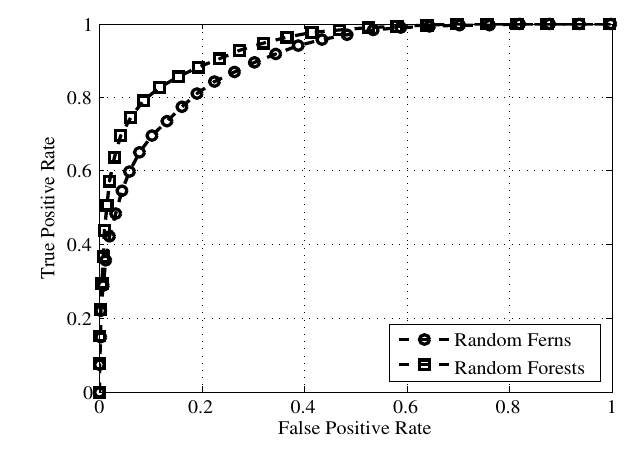
\includegraphics[height=6.5cm]{pics/ferns&forests.png}
		\caption{Porovnanie klasifikátorov Random Forest a Random Ferns.
		 \cite{vieriu2014real}}
		\label{pic-ferns&forests}
	\end{center}
\end{figure}

Podľa článku navrhnutá metóda používa pohľad na tvár spredu a je použiteľná v reálnom čase (30 fps), kvôli rýchlosti výpočtu Random Forest.\\

V článku \cite{joosten2015voice} popisujú a testujú metódu VVAD založenú na časopriestorových Gáborových filtroch (angl. Spatiotemporal Gabor filters), ktorá podľa autorov nebola nikdy predtým na VVAD použitá.
Používajú dve dátové sady: CUAVE - obsahuje nahrávky reči pri pohľade spredu aj z profilu a LIVER - obsahuje nahrávky vyslovovania holandského slova "liver" pri pohľade spredu.
Ich metóda sa skladá z 2 fáz: 
\begin{itemize}
	\item fáza predspracovania - aplikovanie časopriestorových Gáborových filtrov na zistenie energií v konkrétnych rýchlostiach (jeden z parametrov časopriestorových Gáborových filtrov),
	\item agregačná a klasifikačná fáza vytvárajúca sumáciu a klasifikátor, na priradzovanie agregovaných energetických hodnôt do binárnych tried (SPEECH a NON-SPEECH).
\end{itemize}
Nimi navrhnutú metódu porovnávajú s 2 referenčnými metódami - metódou založenou na rozdieloch snímok a metódou založenou na štandardných Gabor filters. 
Ich metóda bola v skoro všetkých prípadoch lepšia ako referenčné metódy. 
Niektoré porovnania je možné vidieť na obrázku \ref{pic-joosten2015voice}.

\begin{figure}[H]
	\begin{center}
		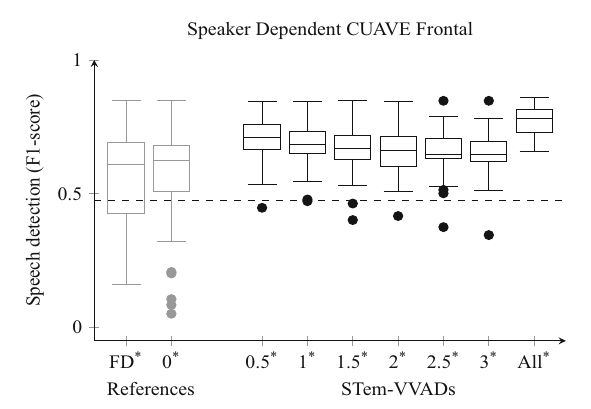
\includegraphics[height=6.5cm]{pics/cuaveFrontal.png}
		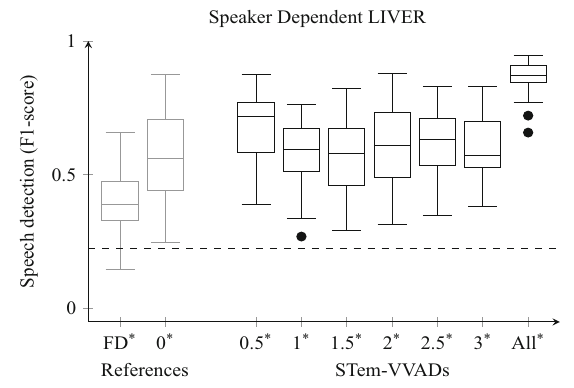
\includegraphics[height=6.5cm]{pics/liver.png}
		\caption{Porovnanie referenčných metód založených na rozdieloch snímok (FD*) a štandardných Gabor filters (0*) s metódou založenou na časopriestorových Gáborových filtroch s rôznymi parametrami rýchlosti (0,5*, 1*, 1,5*, 2*, 2,5*, 3*, All*).
		 \cite{joosten2015voice}}
		\label{pic-joosten2015voice}
	\end{center}
\end{figure}

Metóda z článku \cite{joosten2015voice} funguje pri pohľade spredu aj z profilu.
V článku sa nepíše nič o rýchlosti ich riešenia.\\

\chapter{Návrh riešenia}
Po preštudovaní uvedených článkov, sa ako najpoužiteľnejšie riešenie pre VVAD javí sledovať zmeny pohybu pier popísanú v článku \cite{aoki2007voice}. 
V článku sa nepíše nič o rýchlosti nimi vytvoreného riešenia EBGM na detekciu pier v obraze a riešenie asi nebude fungovať v reálnom čase. 
Naše riešenie bude musieť v reálnom čase fungovať, keďže zapínanie a vypínanie mikrofónu pri videohovore si to vyžaduje. 
V nasledujúcej časti opíšeme články zaoberajúce sa detekciou bodov na tvári.\\

\section{Detekcia bodov na tvári - VVAD}

V článku \cite{ranjan2017hyperface} prezentujú algoritmus na simultánnu detekciu tvárí, bodov na tvári, pozíciu (otočenie) tváre (hlavy) a rozoznávanie pohlavia s použitím DCNN. 
Uvádzajú dve verzie ich algoritmu nazývaného HyperFace:
 \begin{itemize}
\item HyperFace-ResNet, krotý je postavený na modeli ResNet-101 a prináša značné zlepšenie výkonu algoritmu,
\item Fast-HyperFace, ktorý používa rýchlejší detektor tvárí na zrýchlenie algoritmu.
\end{itemize}
Na obrázku \ref{pic-ranjan2017hyperface-siet} je architektúra siete HyperFace. 

\begin{figure}[H]
	\begin{center}
		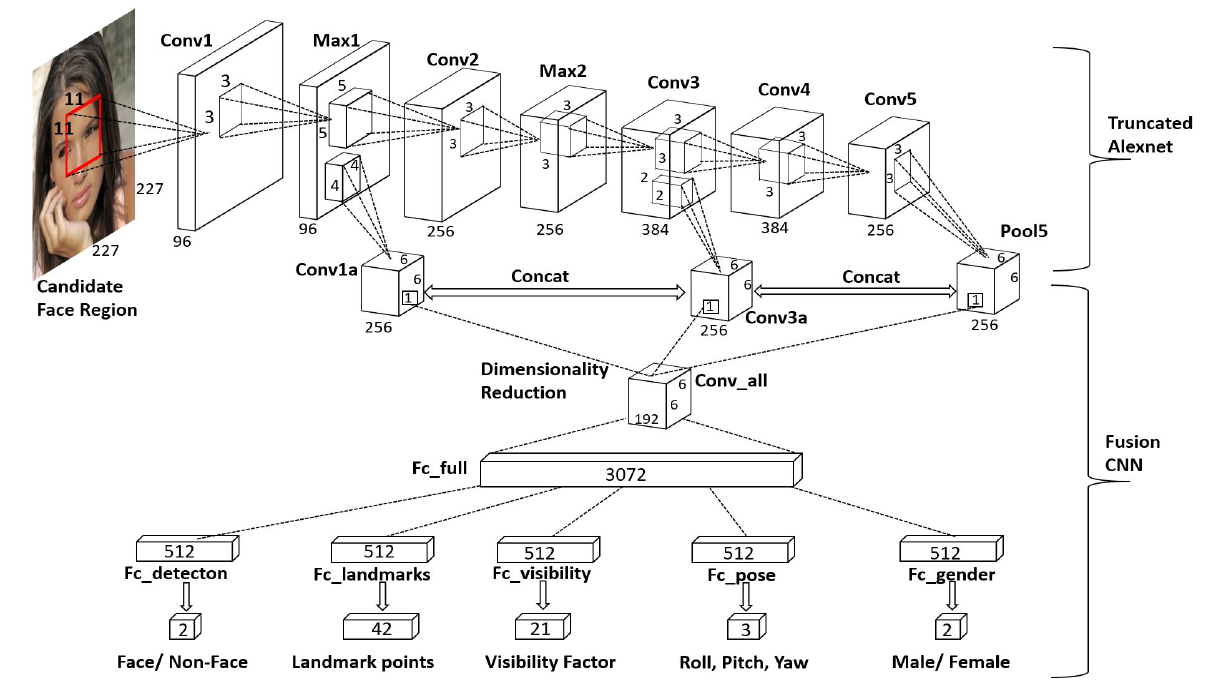
\includegraphics[height=7.5cm]{pics/pic-ranjan2017hyperface-siet.png}
		\caption{Architektúra DCNN HyperFace. 
		 \cite{ranjan2017hyperface}}
		\label{pic-ranjan2017hyperface-siet}
	\end{center}
\end{figure}

Kvôli testovaniu na rôznych dátových sadách trénovali sieť pre rôzne počty bodov (21, 68, ...) na tvári. 
Ukážka výsledkov algoritmu je na obrázku \ref{pic-pic-ranjan2017hyperface-xichty.png}.

\begin{figure}[H]
	\begin{center}
		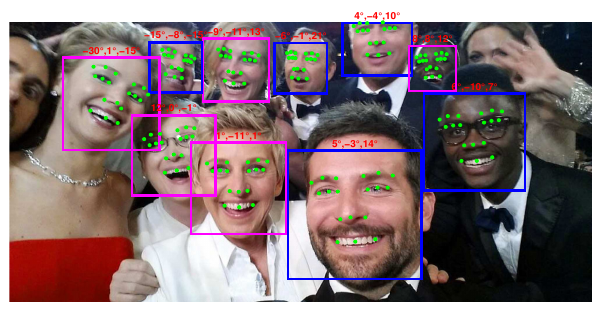
\includegraphics[height=6cm]{pics/pic-ranjan2017hyperface-xichty.png}
		\caption{Algoritmus simultánne deteguje tváre, body na tvári (zelené body), pohlavie (modrý štvorec - muž, ružový štvorec - žena) a pozíciu tváre (červené čísla nad štvorcami - priečny sklon, pozdĺžny sklon a zatočenie).  
		 \cite{ranjan2017hyperface}}
		\label{pic-pic-ranjan2017hyperface-xichty.png}
	\end{center}
\end{figure}

Práca \cite{kazemi2014one} popisuje detekciu bodov na tvári pomocou súboru regresných stromov v reálnom čase. 
Na obrázku \ref{pic-oneMsBody.png} sú výsledky algoritmu na testovacej dátovej sade.

\begin{figure}[H]
	\begin{center}
		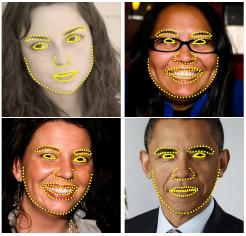
\includegraphics[height=6cm]{pics/oneMsBody.png}
		\caption{Testovacie výsledky algoritmu používajúceho náhodné regresné stromy na nájdenie 194 bodov na tvári. 
		 \cite{kazemi2014one}}
		\label{pic-oneMsBody.png}
	\end{center}
\end{figure}

Pre náš problém sa javí riešenie z článku \cite{kazemi2014one} ako lepšie, keďže už názov článku hovorí o jeho rýchlosti (One millisecond face alignment with an ensemble of regression trees). 
Ďalšou výhodou tohoto riešenia je to, že je implementované v knižniciach Dlib a OpenCV.

(K tomuto článku budem neskor chcieť spísať matematiku, keďže ho v diplomke najviac používam)

\section{Existujúce implementácie}
V tejto podkapitole popíšeme existujúce knižnice (implentácie), ktoré sa zaoberajú detekciou tváre a bodov na nej.

\subsection{Intel RealSense}
V roku 2018 predstavil Intel prvé hĺbkové kamery RealSense.
K týmto kamerám vydal SDK \cite{realsensedis} pre operačný systém Windows. 
Toto SDK dokázalo v obmedzenej miere pracovať aj s bežnou webovou kamerou. 
Dostupná bola pre nás dôležitá metóda detekcie bodov na tvári. 
Ukážka funkcionality SDK je na obrázku \ref{pic-realsensedis}.

\begin{figure}[H]
	\begin{center}
		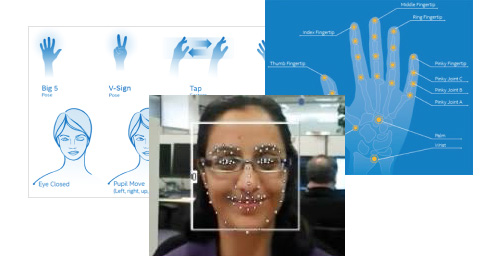
\includegraphics[height=5.5cm]{pics/realsensedis.jpg}
		\caption{Prvé SDK k Intel RealSense dokázalo sledovať ruku a prsty, analyzovať tvár, rozpoznávať reč a. i.
		 \cite{realsensedis}}
		\label{pic-realsensedis}
	\end{center}
\end{figure}

Existujú 2 dôvody, prečo toto riešenie nie je pre nás vhodné: 
\begin{itemize}
	\item podporovaný bol len operačný systém Windows - naše riešenie má byť multiplatformové,
	\item vývoj SDK bol zastavený.
\end{itemize}
Toto SDK bolo nahradené novým multiplatformovým SDK \cite{realsensenew}, ktoré už ale nevie pracovať s bežnou webovou kamerou. 

\subsection{Knižnica OpenCV}
OpenCV\cite{openCv} (Open Source Computer Vision Library) je multiplatformová knižnica zameraná na počítačové videnie.
V knižnici OpenCV je implementovaná detekcia tvárí a aj detekcia bodov na tvári z článku \cite{kazemi2014one}. 
Prečo nepoužijeme knižnicu OpenCV si popíšeme v kapitole \ref{OpenCVvsDlibNadpis}. 
Ukážku detekcie je možné vidieť na obrázku \ref{pic-openCv}. 

\begin{figure}[H]
	\begin{center}
		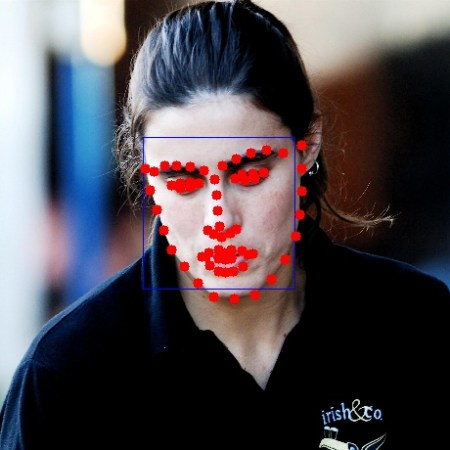
\includegraphics[height=5cm]{pics/openCv.jpg}
		\caption{Ukážka výsledku detekcie bodov na tvári pomocou knižnice OpenCV.
		 \cite{openCv}}
		\label{pic-openCv}
	\end{center}
\end{figure}

\subsection{Knižnica Dlib} \label{DlibNadpis}
Dlib\cite{dlib} je moderná multiplatformová knižnica obsahujúca nástroje pre strojové učenie a vytváranie komplexného softvéru v jakyku C++. 
Ako sme spomínali v pred\-chá\-dza\-jú\-cej podsekcii v knižnici Dlib je implementovaná detekcia bodov na tvári z článoku \cite{kazemi2014one}. 
Ukážka detekcie bodov na tvári pomocou knižnice Dlib je na obrázku \ref{pic-dlibUkazka}.

\begin{figure}[H]
	\begin{center}
		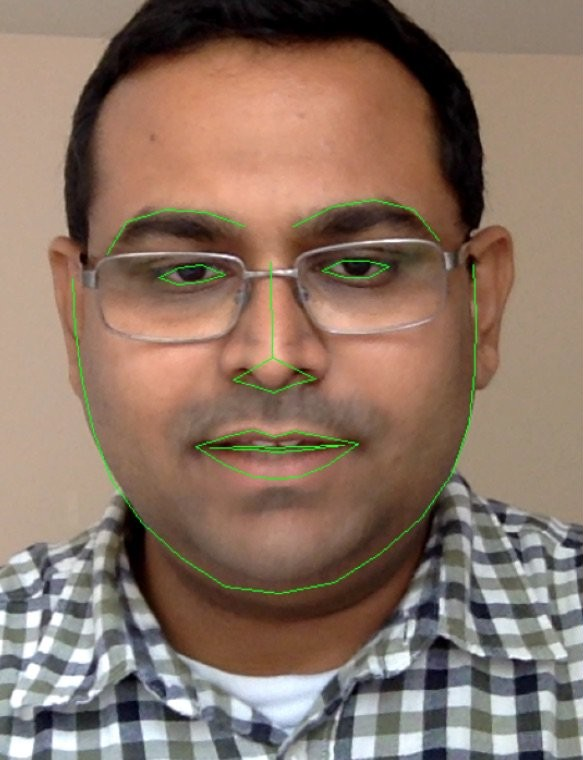
\includegraphics[height=5cm]{pics/dlib.jpg}
		\caption{Detekcia detekcie 68 bodov na tvári pomocou knižnice Dlib.
		 \cite{dlibUkazka}}
		\label{pic-dlibUkazka}
	\end{center}
\end{figure}

\subsection{Porovnanie knižní OpenCV a Dlib} \label{OpenCVvsDlibNadpis}
V oboch knižniciach je implementovaná detekcia bodov na tvári z článku \cite{kazemi2014one}.
Ako problém ostáva nájdenie tváre v obraze.
Obe knižnice ponúkajú viacero metód, ktoré tento problém riešia.
Na stránke \cite{OpenCVvsDlib} porovnávajú metódy detekcie tváre v knižniciach OpenCV a Dlib. 
Zameriavajú sa na 4 nasledujúce metódy:
\begin{itemize}
	\item detekcia tváre pomocou Haar Cascade - OpenCV,
	\item detekcia tváre pomocou DNN - OpenCV,
	\item detekcia tváre pomocou HoG - Dlib,
	\item detekcia tváre pomocou CNN - Dlib.\\
\end{itemize}
Popíšeme výhody a nevýhody jednotlivých metod.\\
\\Detekcia tváre pomocou \textbf{Haar Cascade - OpenCV} bola špičkovou od roku 2001, kedy bola predstavená výskumníkmi Violom a Jonesom.\\
\\Výhody:
\begin{itemize}
	\item funguje takmer v reálnom čase na CPU,
	\item jednoduchá architektúra,
	\item deteguje tváre rôznych veľkostí.
\end{itemize}
Nevýhody:
\begin{itemize}
	\item deteguje veľa objektov, ktoré nie sú tvárami,
	\item nefunguje na tvárach, ktoré nie sú pri pohľade spredu,
	\item Nefunguje ani pri čiastočnom zakrytí tváre.\\
\end{itemize}
Detekcia tváre pomocou \textbf{DNN} je v OpenCV implementovaná od verzie 3.3. \\
\\Výhody:
\begin{itemize}
	\item najpresnejšia zo štyroch uvedených metód,
	\item funguje v reálnom čase na CPU,
	\item rozpozná rôzne otočené tváre,
	\item funguje aj pri značnom zakrytí tváre,
	\item deteguje tváre rôznych veľkostí.
\end{itemize}
Nevýhody:
\begin{itemize}
	\item žiadne, až na tú, že nasledujúca metóda je rýchlejšia.\\
\end{itemize}
Detekcia tváre pomocou \textbf{HoG} je široko používaný model v knižnici Dlib založený na HoG a SVM.\\
Výhody:
\begin{itemize}
	\item najrýchlejšia zo štyroch uvedených metód na CPU,
	\item funguje veľmi dobre pri pohľade na tvár spredu a mierne zboka,
	\item jednoduchý a nenáročný model v porovnaní s ostatnými,
	\item funguje pri čiastočnom zakrytí tváre.
\end{itemize}
Nevýhody:
\begin{itemize}
	\item hlavná nevýhoda je, že metóda nedeteguje malé tváre (cca. 80x80 pixelov),
	\item box ohraničenia tváre často vynecháva čelo a bradu,
	\item nefunguje dobre pri značnom zakrytí tváre,
	\item nefunguje pre pohľad zboka a pre pohľad hore a dole.\\
\end{itemize}
Detekcia tváre pomocou \textbf{CNN} v knižnici Dlib používa Maximum-Margin Object Detector s CNN.\\
Výhody:
\begin{itemize}
	\item funguje pre rôzne orientácie tváre,
	\item metóda je robustná na zakrytie tváre,
	\item funguje veľmi rýchlo na GPU.
\end{itemize}
Nevýhody:
\begin{itemize}
	\item metóda he veľmi pomalá na CPU,
	\item metóda natrénovaná na detekciu tvári väčších ako 80x80 pixelov,
	\item box ohraničenia tváre je ešte menší ako v predchádzajúcom prípade.\\
\end{itemize}

Pre naše potreby je najvhodnejšia metóda detekcie tváre pomocou HoG implementovaná v knižnici Dlib.
Táto metóda nie je najpresnejšia, ale keďže chceme rozpoznávať reč pri videohovore, môžeme predpokladať, že vo väčšine prípadov sa osoba pred kamerou bude pozerať priamo na kameru (monitor) a tvár  nebude mať ničím zakrytú.
To, že metóda má problém s malými tvárami tiež pre nás nie je problém, lebo pri videohovore predpokladáme, že tvár nebude ďaleko od kamery.
Zo spomínaných metód je jednoduchá, nenáročná a na CPU najrýchlejšia, čo je veľmi dobré, lebo kladieme veľký dôraz na to, aby naše riešenie fungovalo v reálnom čase.
Porovnanie rýchlosti jednotlivých metód je uvedené na obrázku \ref{pic-face-detection-speed-comparison}.

\begin{figure}[H]
	\begin{center}
		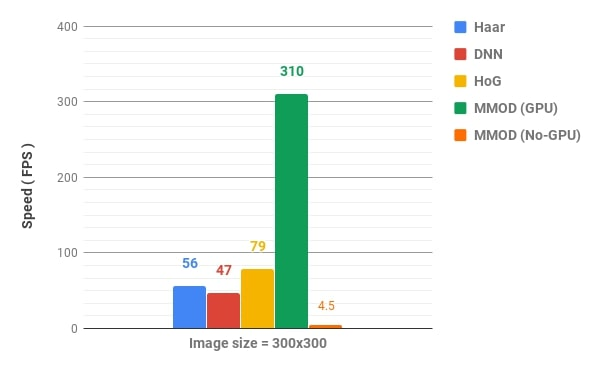
\includegraphics[height=6cm]{pics/face-detection-speed-comparison.jpg}
		\caption{Porovnanie rýchlosti štyroch popísaných metód.
		 \cite{OpenCVvsDlib}}
		\label{pic-face-detection-speed-comparison}
	\end{center}
\end{figure}

\section{Detekcia reči zo zvuku - AVAD}
Detekcia reči z videa nemusí byť pre naše potreby dostatočná. V nasledujúcej časti si popíšeme prácu zaoberajúcu sa detekciou reči zo zvuku.\\

V práci \cite{moattar2009simple} predstavujú takmer ideálny AVAD algoritmus, ktorý je ľahký na implementáciu a robustný vzhľadom na šum.
Pri detekcii využívajú 3 rozdielne vlastnosti pre každú zvukovú snímku: energiu, spektrálnu rovinnosť (Spectral Flatness) a najdominantnejšiu frekvenčnú zložku.
Pre každú z týchto vlastností sa zvolí prah a pre každú zvukovú snímku sa rátajú tieto 3 vlastnosti.
Ak hodnota ktorejkoľvek vlastnosti bude väčšia ako prah prehlási sa aktuálna zvuková snímka za snímku s rečou.
Prahy sa dynamicky menia počas behu algoritmu vzhľadom na predchádzajúce zvukové snímky.
Ukážka vypočítaných vlastností na zvukovom súbore pomocou algoritmu z \cite{moattar2009simple} je na obrázku \ref{pic-avad}.

\begin{figure}[H]
	\begin{center}
		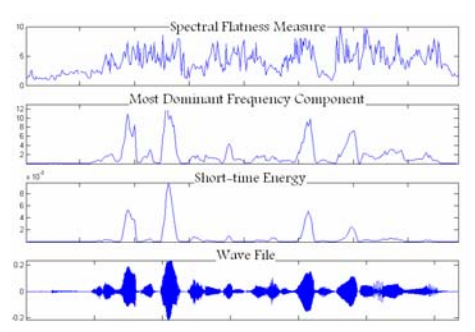
\includegraphics[height=6cm]{pics/avad.png}
		\caption{Ukážka vypočítaných vlastností na zvukovom súbore bez šumu.
		 \cite{moattar2009simple}}
		\label{pic-avad}
	\end{center}
\end{figure}

\section{VAD spojením AVAD a VVAD a vytvorenie knižnice}
Výstupom tejto diplomovej práce by mal program schopný zistiť, či používateľ počas videohovoru rozpráva alebo nerozpráva. 
Na to chceme použi kombináciu metód VVAD a AVAD. 
Kombinácia metód je dôležitá v rôznych prípadoch. 
AVAD je dôležitá keď používateľ nemá webovú kameru, nie je ho na obraze vidieť, v miestnosti je zlé svetlo a. i.
VVAD je dôležitá v prípade nemožnosti detekcie zo zvuku, napríklad kvôli šumu alebo rušivému rozprávaniu inej osoby.

Výstup z práce by mal mať formu dynamickej multiplatformovej C++ knižnice. 
V knižnici by mala byť implementovaná metóda, ktorej vstupom by mali byť dve polia. 
Jedno pole s video snímkou a druhé so zvukovou snímkou.
Výstup metódy by mal záležať od vstupných polí nasledovne:
\begin{itemize}
	\item ak sú obe polia nenulové, metóda by mala vrátiť či bola detegovaná reč, či bola detegovaná zo zvuku alebo videa, pozíciu tváre ak bola detegovaná, a. i., 
	\item ak je pole so zvukovou snímkou nulové a s video snímkou nenulové, či bola detegovaná reč z videa, pozíciu tváre ak bola detegovaná, a. i.,
	\item ak je pole so zvukovou snímkou nenulové a s video snímkou nulové, či bola detegovaná reč zo zvuku, a. i.
\end{itemize}
Takýmto spôsobom môže byť využitie knižnice väčšie.
Napríklad v prípade nedetegovania tváre sa môže znížiť kvalita prenášaného obrazu pri videohovore, čím sa zníži záťaž procesora aj sieťovej linky.

\chapter{Implementácia a testovanie}
V tejto kapitole popíšeme implementáciu nami navrhnutého riešenia VAD v C++ knižnici.

\section{Použitý hardware a software}
Implementácia a testovanie prebiehali na notebooku Asus Zenbook UX305FA (Intel Core M 5Y10, 8GB RAM) a na počítači HP Z240 ( Intel Xeon E3-1245, 16GB ram)
Pre testovanie sme používali webovú kameru LifeCam Cinema.
Vyvíjali sme jazyku C++, ktorý je najvhodnejší pre prácu s videom.
Používali sme knižnice OpenCV, Dlib, SFML.
Ako vývojárske prostredie bol zvolený CLion a buildovali sme pomocou Cmake.

\section{Implementácia VVAD}
Vytvorili sme dynamickú knižnicu s názvom VVAD. 
V hlavičkovom súbore \texttt{VVAD.h} sa nachádzajú definície tried, metód a premenných definovaných v súbore \texttt{VVAD.cpp}.
V hlavičkovom súbore sú definované dve triedy: \texttt{VVAD} a  \texttt{Output}.
Trieda \texttt{VVAD} je hlavnou triedou, ktorá obsahuje verejne metódy:
\begin{itemize}
\item \texttt{Frame} - hlavná metóda, ktorej vstupom je video snímka a výstupom je objekt triedy \texttt{Output}.
\item \texttt{FrameForLearningThreshold} - metóda sa volá na začiatku používania knižnice na určenie prahu. Vstupom metódy je video snímka a výsledným výstupom je prah, pomocou ktorého metóda \texttt{Frame} vyhodnocuje, či vo videosekvencii nastala reč alebo nie.
\item \texttt{SaveThreshodToFile} - metóda uloží prah do súboru určeného reťazcom, ktorý dostane na vstup.
\item \texttt{LoadThresholdFromFile} -  metóda načíta prah zo súboru určeného reťazcom, ktorý dostane na vstup.
\item \texttt{getThreshold} - vráti hodnotu prahu.
\item \texttt{setThreshold} - nastaví hodnotu prahu.
\item \texttt{isCalibrated} - vráti pravdivostnú hodnotu, ktorá hovorí, či prah bol nastavený.
\item \texttt{getCalibrated} - nastaví pravdivostnú hodnotu, ktorá hovorí, či prah bol nastavený.
\end{itemize}

Trieda  \texttt{Output} sa používa ako výstup metóda  \texttt{Frame}. Trieda obsahuje nasledujúce privátne premenné, ktoré sú prislúchajúcimi metódami dostupné na čítanie:
\begin{itemize}
\item \texttt{\_talking} - pravdivostná premenná, ktorá ak platí, tak reč bola detegovaná, inak reč detegovaná nebola.
\item \texttt{\_count\_of\_faces} - počet nájdených tvárí.
\item \texttt{\_faces\_positions} - pozície nájdených tvári na snímke, ktorý dostala metóda \texttt{Frame} na vstupe.
\end{itemize}

V nasledujúcej časti popíšeme fungovanie niektorých metód detailne.

\subsection{Metóda \texttt{Frame}}
Zo snímky, ktorú dostane metóda \texttt{Frame} na vstupe sa vytvorí kópia, ktorá sa predspracuje.
Predspracovanie spočíva v zmene rozlíšenia tak, aby šírka snímky bola  720 pixelov (toto predspracovanie budeme nazývať preškálovanie).
Toto rozlíšenie bolo zvolené tak, aby nasledujúca detekcia tváre v snímke bola dostatočne rýchla aj na menej výkonných procesoroch.
Detekcia tváre je presnejšie popísaná v časti \ref{detekciaTvare}.
Výstupom z detekcie tváre je pole pozícií nájdených tvárí v kopijí pôvodnej snímky. 
Následne, ak sa nenašla práve jedna tvár, tak sa daná snímka preskakuje. 
Ak sa našla práve jedna tvár, prebieha detekcia bodov na tvári v pôvodnej snímke. 
Detekcia bodov na tvári je detailne popísaná v časti \ref{detekciaBodov}.
Nájdené body na tvári spracúva metóda \texttt{ComputeDifferenceBetweenRatios}, ktorá je popísaná v časti \ref{pomerPier}.
Nakoniec už len metóda \texttt{CheckSpeechInLastFrames}, vysvetlená v časti  \ref{kontrolaReci}, skontroluje, či nastala reč a podľa toho sa vytvorí objekt triedy \texttt{Output}, ktorý sa dáva na výstup. 
Detailný popis metódy \texttt{Frame} je na obrázku \ref{pic-Frame}.

\begin{figure}[H]
	\begin{center}
		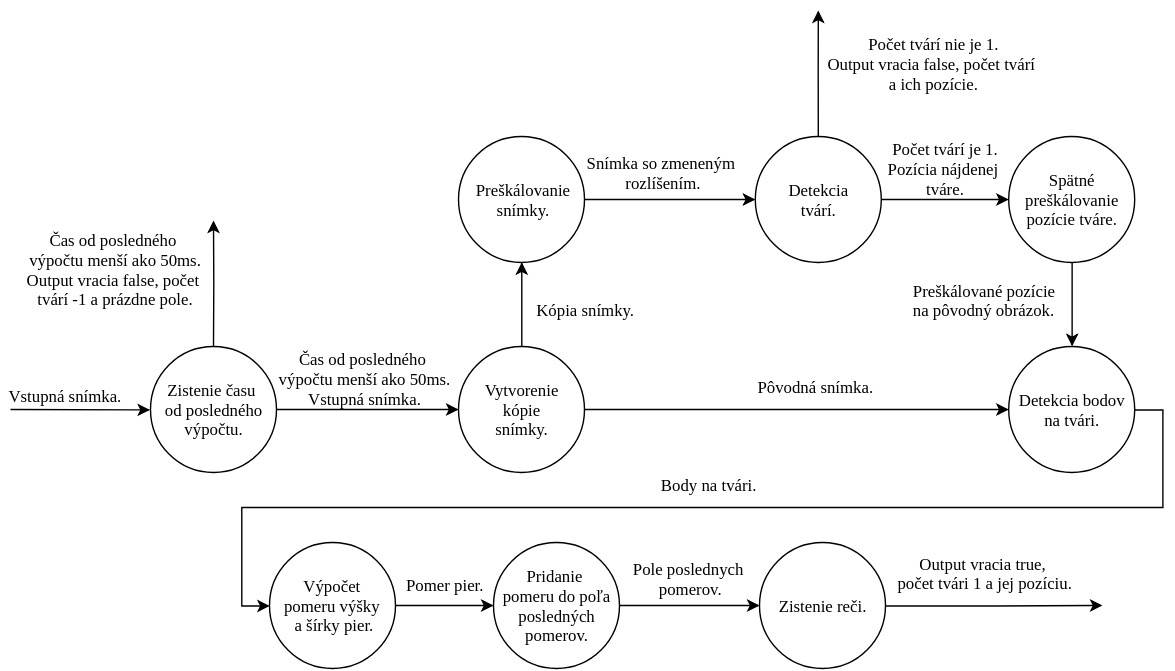
\includegraphics[height=8.7cm]{pics/Frame.jpg}
		\caption{Graf priebehu metódy \texttt{Frame}. Vo vrcholoch sú akcie, ktoré sa vykonávajú, šípky znázorňujú výstupy z akcií.}
		\label{pic-Frame}
	\end{center}
\end{figure}

\subsubsection{Detekcia tváre}\label{detekciaTvare}
Ako sme popísali v časti \ref{OpenCVvsDlibNadpis}, na detekciu tvárí sme použili knižnicu Dlib, konkrétne detekciu tvárí pomocou HoG. 
Táto detekcia je najpomalšia čast celého algoritmu, no aj napriek tomu funguje dostatočne rýchlo na oboch počítačoch, ktoré sme pri implementácií používali.
Dôvodom je to, že detekcia tváre je spúšťaná na preškálovanej snímke.
Pozície tvárí sa po nájdení preškálujú tak, aby boli na správnych miestach v pôvodnej snímke a uložia sa do vektora.

\subsubsection{Detekcia bodov na tvári}\label{detekciaBodov}
Pre detekciu bodov na tvári budeme potrebovať natrénovaný model. 
V príkladových súboroch knižnice sa nachádzajú aj 2 predtrénované modely, ktoré detegujú 68 alebo 5 bodov na tvári. 
Model so 68 bodmi má približne 95MiB, čo je príliš veľa a model s 5 bodmi zas neobsahuje body na perách.
Rozhodli sme sa teda vytvoriť vlastný model, ktorý by mal menšiu veľkosť a bol dostatočne presný pre naše potreby.
Pre trénovanie modelu budeme potrebovať fotografie osôb a k nim súbor s popisom umiestnenia bodov na tvárach (súbory sú štandardne formátu xml, budeme ich preto skrátene nazývať xml súbory).
V príkladových súboroch sa nachádzajú fotografie aj xml súbory pomocou ktorých je možné trénovať model.
Na trénovanie sú určené 4 fotografie s celkovo 18 tvárami.
Na testovanie je určených 5 fotografií s celkovo 25 tvárami.
Pomocou uvedených súborov však nie je možné natrénovať dostatočne presný model.
Na stránke knižnice Dlib sa dá nájsť dátová sada ibug\_300W\_large\_face\_landmark\_dataset, čo je vlastne dátová sada 300-W \cite{ibug} s pridanými zrkadlovo otočenými obrázkami (pri použití dátovej sady  300-W \cite{ibug} žiadajú citovať \cite{sagonas2016300}, \cite{sagonas2013300} a \cite{sagonas2013semi}) 
Dátová sada  300-W \cite{ibug} obsahuje fotografie z dátových sád afw, helen, ibug a lfpw. 
Dátová sada samozrejme obsahovala aj testovaci a trénovací xml súbor s označenými umiestneniami 68 bodov na tvári, pomocou ktorých je možné natrénovať presnejší model.
Trénovací súbor obsahoval 6666 tvári a testovací obsahoval 1008 tvári.
Knižnica Dlib obsahuje nástroj na vytváranie a úpravu xml súborov s informáciami o bodoch na tvárach na fotografiách a aj nástroj na trénovanie a testovanie modelu na základe fotografií a xml súborov.
Pomocou nástroja na prácu s xml súbormi z knižnice Dlib a editora Sublime Text sme upravili počet bodov na tvári v xml súboroch.
Nástroj na trénovanie má možnosť nastaviť parametre trénovania, ako je napríklad hĺbka stromu a. i. (POPIŠ VIAC)
Vytvorili sme 2 nové modely, úpravou xml súborov pre 68 bodový model, odstránením niektorých bodov:
\begin{itemize}
	\item 20 bodový model pier. 
	Ponechali sme len body na perách. 
	Model ale nebol dostatočne presný.
	\item 27 bodový model pier.
	Kvôli zvýšeniu presnosti modelu sme okrem 20 bodov na perách nechali body na spodnej časti uši, bod na brade, nose, medzi očami a vonkajšie krajné body očí.
	Ani tento model nebol dostatočne presný.
\end{itemize}

Keďže sa nám zatiaľ nepodarilo vytvoriť vhodnejší model používali sme 68 bodový model.
(Stale sa snazim vytvorit lepsi model)
Ukážka detekcie modelu so 68 bodmi v obraze z webovej kamery je na obrázku \ref{pic-detekciaKsicht}.

\begin{figure}[H]
	\begin{center}
		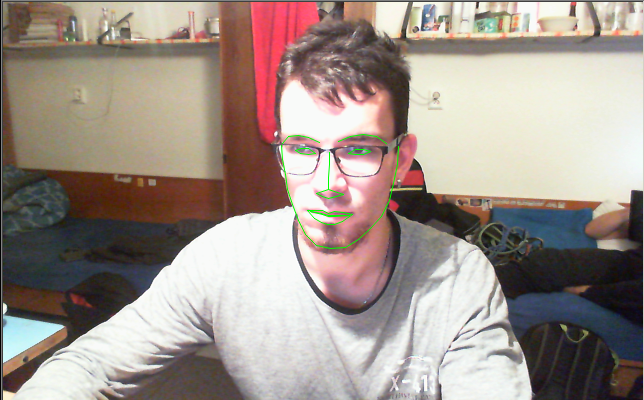
\includegraphics[height=6cm]{pics/detekciaKsicht.png}
		\caption{Ukážka detekcie modelu so 68 bodmi v reálnom čase pomocou knižnice Dlib.}
		\label{pic-detekciaKsicht}
	\end{center}
\end{figure}

Uložený natrénovaný model sa načíta pri volaní konštruktora triedy \texttt{VVAD}.
Vytvorí sa objekt triedy \texttt{shape\_predictor} z knižnice Dlib, ktorého metóda na detekciu bodov na tvári sa volá po zdetegovaní tváre.
Metóda dostane na vstup pôvodnú snímku a pozíciu zdetegovanej tváre a na výstup vráti objekt triedy \texttt{full\_object\_detection}, ktorý obsahuje pozíciu tváre a vektor bodov na tvári.

\subsubsection{Pomer pier}\label{pomerPier}
V metóde \texttt{ComputeDifferenceBetweenRatios} je implementovaná časť práce \cite{aoki2007voice}.
Z dvadsiatich bodov na perách sa najprv zrátajú pozície bodov z ktorých sa bude rátat pomer výšky a šírky pier:
\begin{itemize}
\item horný - zoberú sa 4 body v hornej časti pery, z ktorých sa spraví primer,
\item dolný - zoberú sa 4 body v dolnej časti pery, z ktorých sa spraví primer,
\item pravý - zoberú sa 2 body v hornej časti pery, z ktorých sa spraví primer,
\item ľavý - zoberú sa 2 body v hornej časti pery, z ktorých sa spraví primer.
\end{itemize} 
Ukážku popísaných bodov je možné vidieť na obrázku \ref{pic-bodyPomeru}.
Z pravého a ľavého boud sa vyráta šírka pier a z horného a dolného bodu výška.
Následne sa vypočíta pomer výšky a šírky a zráta sa absolútna hodnota rozdielu aktuálneho pomeru a pomeru z predchádzajúcej snímky. 
Pomocou metódy \texttt{ShiftAndAddRatioDifference} sa vypočítaná absolútna hodnota uloží do 10 prvkového posuvného poľa.
Ako toto desať prvkové pole funguje, je vysvetlené na obrázku \ref{pic-vysvetleniePosuvnehoPola}.

\begin{figure}[H]
	\begin{center}
		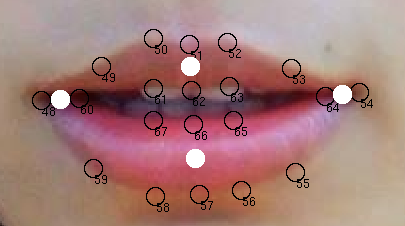
\includegraphics[height=5cm]{pics/peryBodyUpravene.png}
		\caption{Ukážka bodov na perách. Horný biely bod je priemer žiernych bodov 50, 52, 61, 63, biely dolný 67, 65, 58, 56, biely pravý 64 a 54 a biely ľavy 48 a 60.}
		\label{pic-bodyPomeru}
	\end{center}
\end{figure}

\begin{figure}[H]
	\begin{center}
		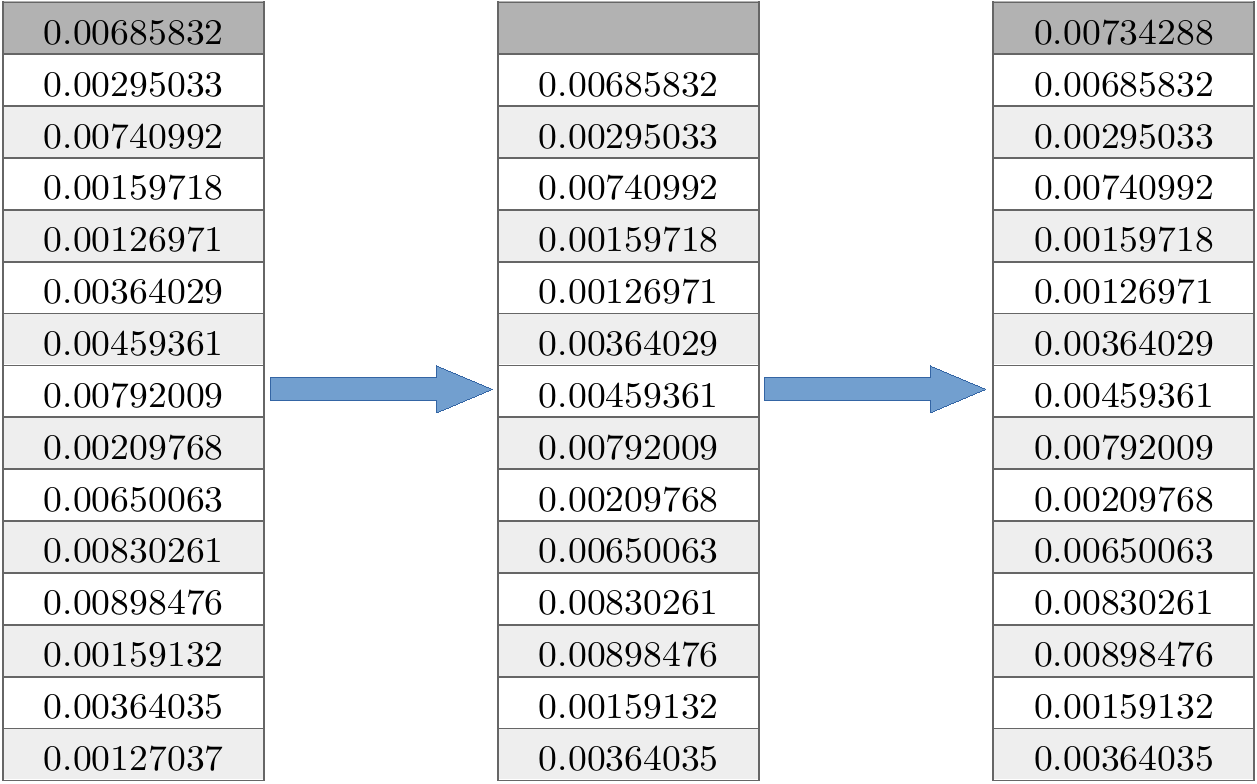
\includegraphics[height=5cm]{pics/vysvetleniePosuvnehoPola.png}
		\caption{Vysvetlenie posuvného poľa.
		Pri zrátaní abslútnej hodnoty rozdielov pomerov sa posunú hodnoty v poli a nová hodnota sa vloží na prázdne miesto. 
		Takto si pamätáme posledných desať rozdielov pomerov.}
		\label{pic-vysvetleniePosuvnehoPola}
	\end{center}
\end{figure}

\subsubsection{Kontrola reči}\label{kontrolaReci}
Po pridaní hodnoty do posuvného poľa sa v metode \texttt{Frame} zavolá metóda \texttt{Check\-Speech\-InLastFrames}.
V nej sa skontroluje, či sa v poli nachádza hodnota väčšia ako určený prah.
Ak áno metóda \texttt{Frame} dá na výstup objekt tiedy \texttt{Output} s parametrami pravda, počtom tvári 1 a s pozíciou danej tváre.
Ak nie metóda \texttt{Frame} dá na výstup objekt tiedy \texttt{Output} s parametrami nepravda, počtom tvári 1 a s pozíciou danej tváre.

\subsection{Metóda \texttt{FrameForLearningThreshold}}

\begin{figure}[H]
	\begin{center}
		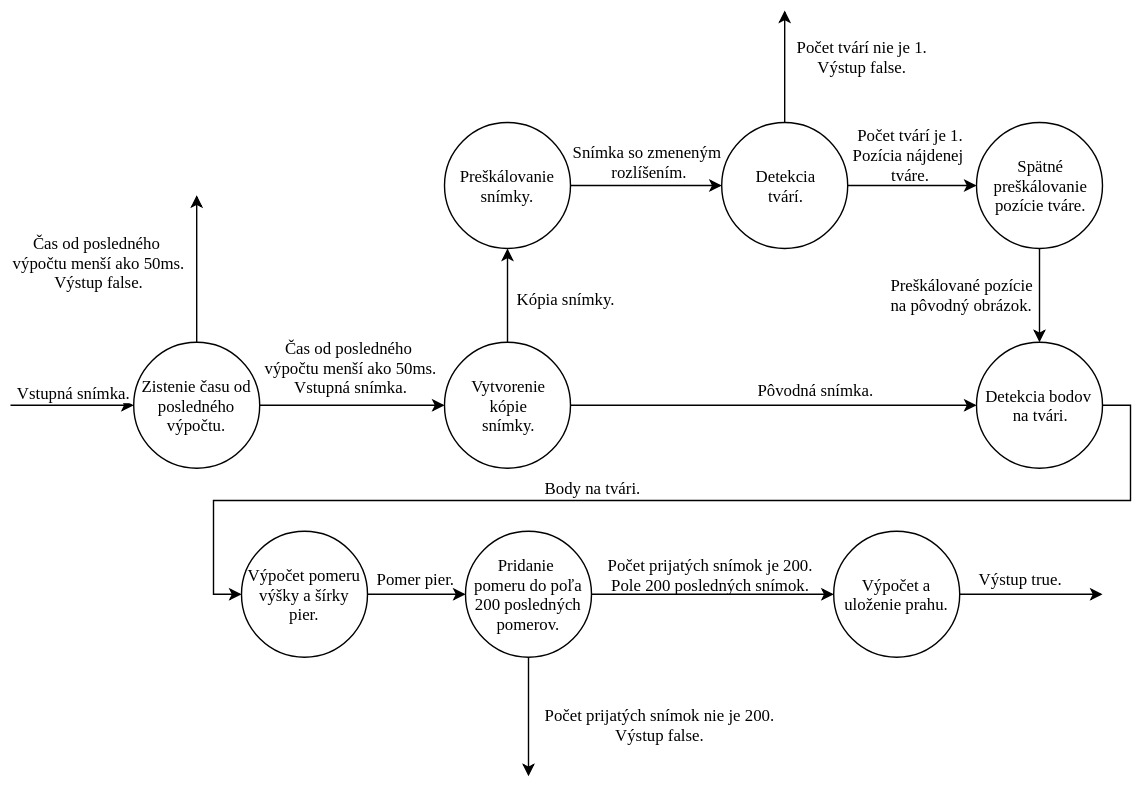
\includegraphics[height=10.3cm]{pics/FrameForLearningThreshold.jpg}
		\caption{Graf priebehu metódy \texttt{FrameForLearningThreshold}. Vo vrcholoch sú akcie ktoré sa vykonávajú, šípky znázorňujú výstupy z akcií.}
		\label{pic-Frame}
	\end{center}
\end{figure}

\section{Implementácia AVAD}
Pri implementovaní AVAD sme používali knižnicu SFML \cite{SFML}.
Pracuje sa na tom...

\subsection{Testovanie}

Navrhnutú metódu sme testovali na viacerých videách s rozprávajúcou osobou.
Po niekoľkých videách sme odhadli vhodnú hodnotu prahu. 
Takto zvolený prah však nemusí vždy správne určiť, či prebieha reč alebo nie.
(prah asi bude dobre upravovat v case - to este musim domysliet)
Na obrázku \ref{pic-spravneRozpoznanie} je graf rozdielu pomerov, prislúchajúci videu, kde osoba na zaciatku rozprávala a ku koncu nie. 
V tomto prípade navrhnutá metóda správne vyhodnotila priebeh reči.

\begin{figure}[H]
	\begin{center}
		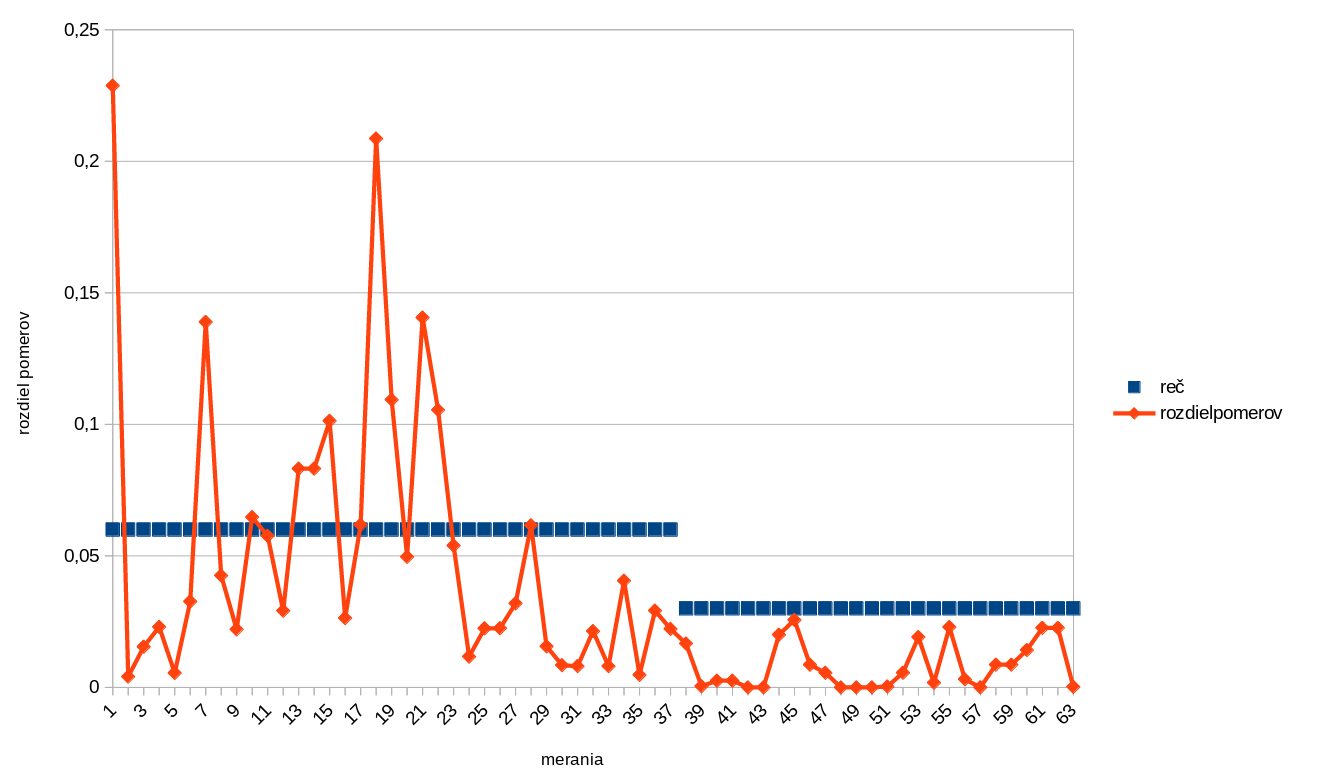
\includegraphics[height=7cm]{pics/spravneRozpoznanie.png}
		\caption{Korektná detekcia reči pomocou navrhnutej metódy VVAD.
		Červené body sú absolútna hodnota rozdielov pomerov 2 po sebe idúcich meraní. 
		Modrá čiara vo výške 0,6 znamená, že reč bola detekovaná a vo výške 0,3, že nebola detekovaná.}
		\label{pic-spravneRozpoznanie}
	\end{center}
\end{figure}

Na obrázku \ref{pic-nespravneRozpoznanie} je graf rozdielu pomerov, prislúchajúci videu s inou osobou, ktorá na začiatku nerozprávala, potom rozprávala a ku koncu opäť nerozprávala. 
Približne v strede grafu je modrá čiara na úrovni 0,3, čo znamená, že metóda vyhodnotila túto časť videa ako časť kde osoba nerozpráva, čo nie je korektné.

\begin{figure}[H]
	\begin{center}
		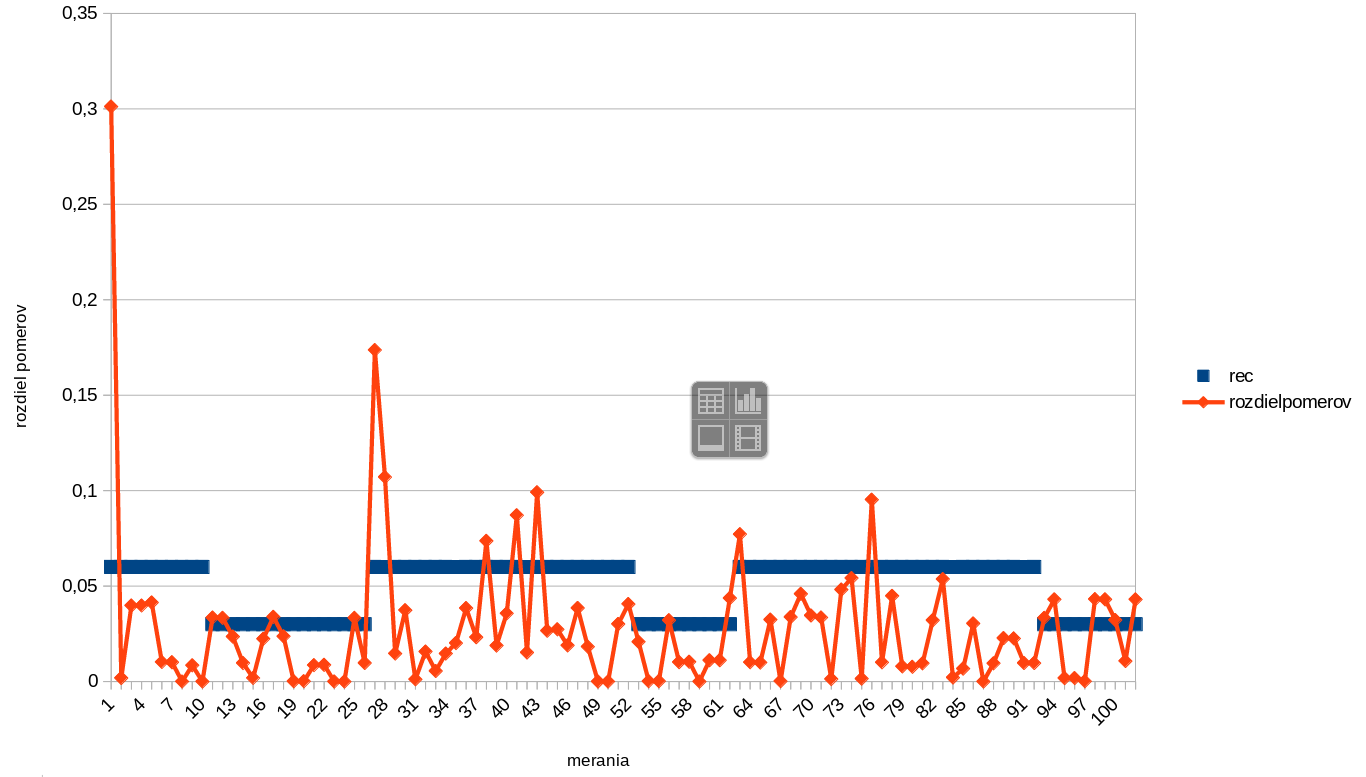
\includegraphics[height=7cm]{pics/nespravneRozpoznanie.png}
		\caption{Nepresná detekcia reči pomocou navrhnutej metódy VVAD.
		Červené body sú absolútna hodnota rozdielov pomerov 2 po sebe idúcich meraní. 
		Modrá čiara vo výške 0,6 znamená, že reč bola detekovaná a vo výške 0,3, že nebola detekovaná.}
		\label{pic-nespravneRozpoznanie}
	\end{center}
\end{figure}